\documentclass[../../main]{subfiles}

\renewcommand\thesection{\arabic{section}}


\begin{document}

\section{Environment Monitoring and Control Unit} \label{sec:}

\textsc{Emcu} takes care of everything related to the environment of
the seedling. It helps to mimic the preferable conditions of the
seedling in the insides of the incubator, even though the outsides
possess a harsh environment. EMCU is further classified into different
systems. In the following chapters we will get familiarized with most
of these systems and their different aspects.

% \textsc{Emcu} tries to monitor and control various aspects that affects the
% seed growth. Inorder to accomplish that, \textsc{Emcu} needs to
% \emph{interface} various \emph{actuators} and \emph{sensors}. As a matter of
% fact, the sheer amount of \emph{actuators} and \emph{sensors} required to
% achieve this exceeds the total number of GPIOs\footnote{General Purpose Input
% Output pins.} \esp has. In order to \emph{synchronize} all of the
% \emph{subsystems}, \esp needs an \emph{external subsystem} to control all the
% other \emph{subsystems}, an \textsc{Auxiliary System} as we will be calling
% this \emph{external system}, in this entire document.
%
% Apart from the \textsc{Auxiliary System}, the \textsc{Emcu} consists of $5$
% other main \emph{hardware subsystems}.

%% PIC

% \begin{figure}
%     \centering
%     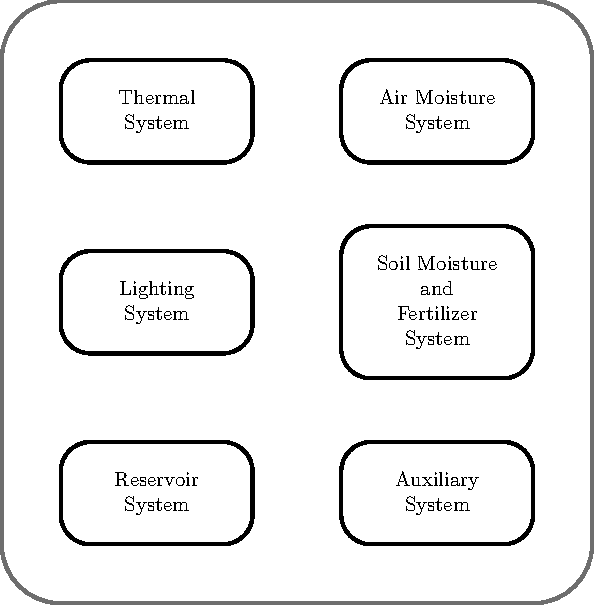
\includegraphics [
%         max width = 0.5\textwidth,
%         max height = 0.5\textheight,
%         \IGXDefaultOptionalArgs,
%     ] {pics/endAbsSubsystems.pdf}
%     \captionof{figure} {Hardware Subsystems of Incubator.}
%     \label{fig:absSubsystems}
% \end{figure}



%Thermal System%
%Air Moisture System%
%Lighting System%
%Soil Moisture and Fertilizer System%
%Reservoir System%

%% Communication System

%\subsection{Thermal System}
%
%The \emph{thermal system} as the name suggests, takes care of the temperature inside
%the incubator. There are several

\end{document}
